% !TeX spellcheck = en_GB

\begin{comment}
\begin{itemize}
	\item goal == identify threats/attacks in KNX networks
	\item only a part in defence system
	\item attempt is to fit anomaly detection model best to normal behaviour in the network
	\item therefore it also necessary to account for usage cycles/periods/seasons of building usage
	\subitem since it has a direct impact on the bus activity
	\item changes in usage may be identified as anomaly -> which could also be interesting
	\subitem reflect e.g. physical intrusion, not intended use of the building, etc.
	\item ...
	
	\item novelty == in-band monitoring
		\subitem mention problems
	\item basic architecture according to \textcite{Pan2014}
	\item \enquote{Intrusion detection systems (IDSs) “are based on the beliefs that an intruder’s behavior will be noticeably different from that of a legitimate user and that many unauthorized actions are detectable” [2].} \parencite{Mukherjee1994,Yang2006}
	\item focus on inside attacks \enquote{The intruder has been granted access to the network and may have some knowledge about the network architecture, including where their targeted files or system vulnerabilities.} \parencite{Yang2006}
	
	\item only high level anomaly detection is done by algorithms, since simple measurements can be evaluated in Grafana
		\subitem e.g. change in packets per seconds
\end{itemize}
\end{comment}

\todo{better intro sentence?}
The overall goal is to identify and react to threats and attacks within \gls{bas} networks, which are indicated by malicious traffic.
This thesis attempts to solve on part of the problem by providing a framework to detect anomalies in those networks.
However, it is not part of this concept to identify the kind of attack, nor to distinguish it from abnormal network activity, caused by a rapid change of user behaviour.
Also it is to note, that the introduced system is merely a part in the defence line.

The architecture proposed in this section is inspired by \textcite{Pan2014}, with extensions made in regards for scalability and continuous use. (cf. Section~\ref{sec:concept:pipeline})
Opposed to \textcite{Pan2014}, which are using an inductive rule learning algorithm (cf. Chapter~\ref{sec:background:prior-work}), this work employs anomaly detection algorithm, which are able to be trained with unlabelled data sets. (cf. Section~\ref{sec:background:network:novelty})
This decision was made because \gls{bas} are mostly heterogeneous, since every building and its usage is different, compared to the fire detection system used by \textcite{Pan2014}.
Therefore, either the baseline model has to reflect a very broad \emph{normality}, or attacks are modelled as signatures. Later option has the drawback of requiring constant updates. Also a sufficiently large database of common attacks is required in first place.
Neither of these options seemed feasible.
Consequently, relying on anomaly detection algorithms made more sense in the provided context.
Despite anomaly based \glspl{ids} being highly useful in changing environments with possibly unknown threats (cf. Section~\ref{sec:background:network:ids:anomaly}), it is to note that they \enquote{are based on the beliefs that an intruder's behavior will be noticeably different from that of a legitimate user and that many unauthorized actions are detectable}. \parencite{Mukherjee1994,Yang2006}

\todo{better transition}
Further, to enable scalability and on-line detection, the proposed framework was designed around the message-passing design principle.
This allows for an easily scalable deployment, strongly capsules application modules, and handles recovery after crashes without data-loss.
Especially later two are not only desired characteristics of an production system, but also speed up development and testing rapidly.

Another novelty, compared to prior examples in literature (cf. Chapter~\ref{sec:background:prior-work}), is the focus of passing the flow-data from the Agent to the collector in-band. By doing so, there is no requirement for additional network wiring, which results in easier and possibly cheaper deployment for Agents across the network.
However, this also introduces new challenges, as the aggregated flow data needs to fit within a relatively small data package, in case of \gls{knx} 255 Bytes. (cf. Section~\ref{sec:background:bas:knx:proto:data})
Also, the collector and the analytical modules need to account for the fact, that no traffic from the Agents can pass the network, e.g. due to \gls{dos} attacks.

\todo{challenge, since there are no real flows.}
Another challenge arises from the nature of \gls{bas} itself. Unlike \gls{scada} networks, where actions follow strict rules and orders and are therefore highly predictable or \gls{ip} networks, which mostly transport connection based traffic. The communication in \gls{bas} networks consists of many short self-contained commands, which occur in seemingly random fashion, since they are mainly triggered by human behaviour. This includes (light) switches, \gls{pir} motion detectors, or door sensors.
Due to the fact, that most telegrams are short commands or status reports from sensors, there are no elaborative connection based communication flows in \gls{bas} networks, thus rendering flow-monitoring less useful.
To counteract this \hint{somewhat special} characteristic, the idea of flow-monitoring is interpreter rather liberal. 
Namely, by focussing more statistics of all telegrams or packets during a specific synchronised time window, instead of tracking individual flows, which also requires less resources on the Agent.
\todo{mention, that also rapid change in user behaviour will trigger anomaly detection}

As already mentioned, this system can merely be a part of comprehensive security system. Acknowledging this fact, the outlier detection algorithms focus mainly on high level anomaly detection, as simpler measurements, like a change in telegrams per seconds, can be simply evaluated in a monitoring and alerting frontend like \gls{grafana}.

\section{Monitoring Pipeline}
\label{sec:concept:pipeline}

\begin{comment}
\begin{itemize}
	\item goal == monitor KNX traffic
	\item notion of \emph{project} is used to differentiate unique, not comparable KNX networks. Can be seen as a common prefix for everything which need to be named internally.
	\item monitoring should include the whole network/world view
	\item monitoring needs to be distributed, so Line Couplers can be configured properly
	\item monitoring is done by Agents
	\item Agents will send data gather over a time window to the collector (ref to neflow terminology)
	\item time windows of Agents are synchronised (by the collector) to make data analysis more reliable
	\item Agents send gathered data to collector via KNX network
	\item collector stores windows immediately in InfluxDB
	\item collector checks regularly the InfluxDB, if all Agents send in their time window
	\item if so the collector relays all windows, describing the same time slot (+/- a couple seconds), to the analyser modules
	\item if not all windows are in by specified timeout (10s or so) they are relayed anyway
	\item bundled windows are distributed by pub-sub-server independently to different analytical modules
	\item analytical modules compare the windows to a base-line model (in different fashions)
\end{itemize}
\end{comment}

For the overall goal to identify threats and attacks within \gls{bas} networks by detecting anomalies, a reliable way to monitor packets or telegrams within said networks is required. Further, this data needs to be processed and analysed, for which a data-pipeline seems well suited.
In this section the general structure and flow within this pipeline is presented. (cf. Figure~\ref{fig:concept:architecture})

\begin{figure}[h]
	\centering
	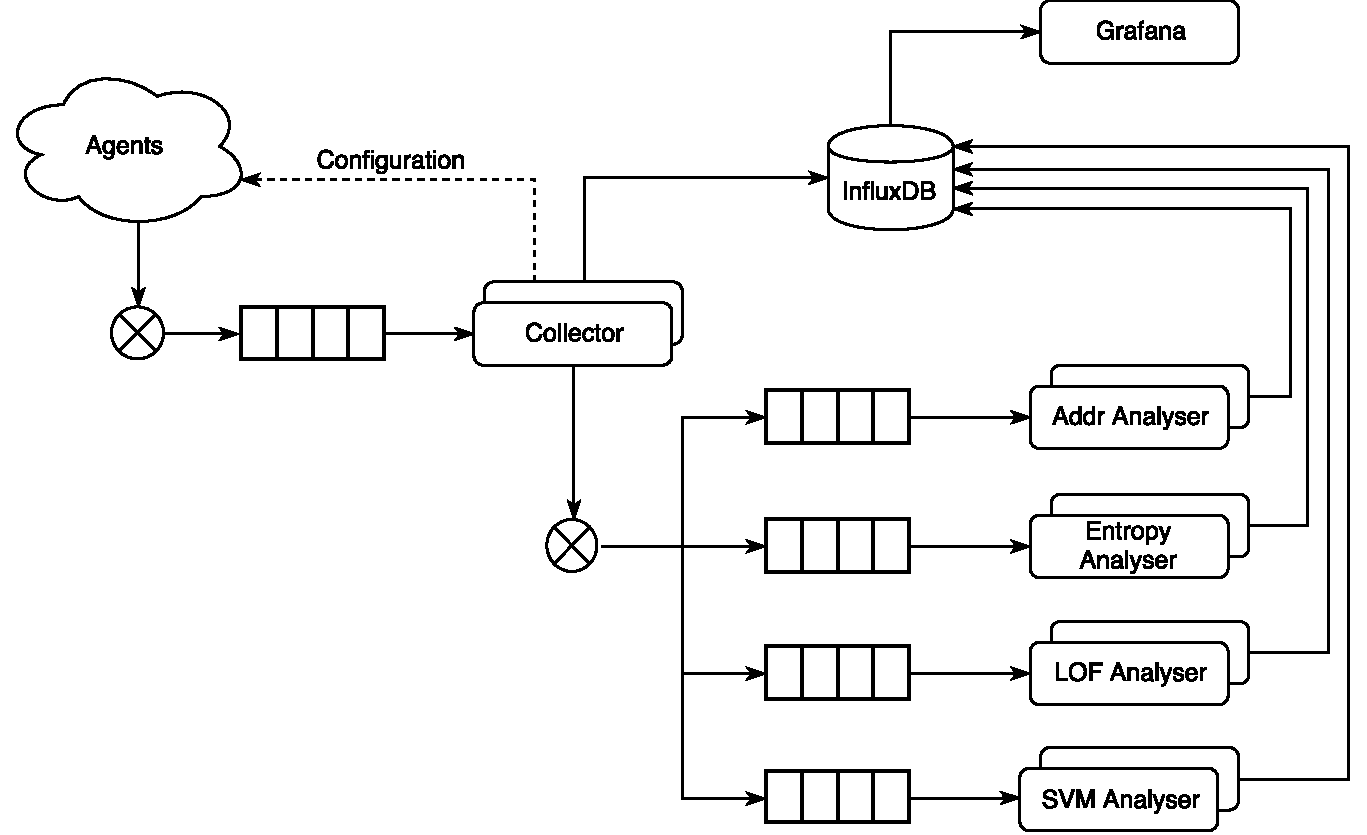
\includegraphics[width=\textwidth]{figures/300-concept-architecture.pdf}
	\caption[Pipeline Architecture]{Architecture of the monitoring pipeline \todo{explain symbols.} \todo{information flow back to agents, for time sync.}}
	\label{fig:concept:architecture}
\end{figure}

Within the here proposed pipeline the notion of a \emph{project} is used to differentiate unique, not comparable \gls{bas} networks, which share the same analytical resources. It can be understood as common prefix for all internal references. (cf. Chapter~\ref{sec:impl})
This is not only a beneficial option, when monitoring multiple networks one the same analytical infrastructure, but also allows for quick testing with different data-sets during development.
Further, all exchanged messages are buffered in queues, to enable easy scaling and recovery after a module or service crashes.
%To further improve use in production, as well as ease of development, ... (RabbitMQ, but this a detail for impl sec)

Following concepts in literature \parencite[cf.][]{Celeda2012,Pan2014} the pipeline is not build around analysing a full-take of traffic within a \gls{bas}, but rather follows the flow monitoring idea. (cf. Section~\ref{sec:background:network:netflow})
However, as stated above (cf. Chapter~\ref{sec:methods},~\ref{sec:concept}), traditional flow monitoring is well suited for \glspl{bas} like \gls{knx}. Therefore, the focus is on general statistical data of all packets or telegrams passing by an Agent within a specific time window.

Since one of the requirements for sufficiently efficient flow-monitoring is to obtain world view (cf. Section~\ref{sec:background:network:netflow},~\ref{sec:methods}), multiple flow monitoring Agents need to be distributed across the \gls{bas} network. Otherwise, network segmentation would be required to be switched off, so a central tapping point could be used for data acquisition.
Whereas this would decrease complexity, it is not advisable since segmentation is one of the fundamental security concepts e.g. in \gls{knx}. (cf. Section~\ref{sec:background:bas:knx:security})
Consequently, a number of Agents, distributed over the whole network, will gather statistical data and send it of to central service -- the Collector.

The Collector is not only responsible for receiving data from Agents and storing them in a database, but also synchronises these windows. Synchronising the windows simplifies the implementation of the analytical modules (cf. Section~\ref{sec:concept:anal}), since they do not need to account for distorted weights, introduced by changing overlaps or lengths of windows sent by the Agents.
This is archived, first of all by waiting until all windows from all Agents have been send to the Collector. Only then they are relayed to the analytical modules as one unit.
However, this only works reliable if the Agents are in sync with each other. If not the Collector would need to compensate for different, changing overlaps. Therefore another task of the Collector service is to ensure the Agents are synchronised, meaning the Agents capture the same length of the of statistical data in the same rhythm without shifting. \alert{rhythm is quite the right thing here, it's more a shift of the length...}
This is archived by communicating back to the Agent modules, regularly updating the \gls{rtc} and important settings like window length and a time point for starting new windows. (shift in time)

Regular two-way communication between Agents and Collector also has the benefit of identifying simple replay attacks (cf. Section~\ref{sec:methods}), since not or wrongly reacting to configuration requests can be detected.
Further, accounting for dynamic configuration of the agents allows for adjusting parameters based on the general network load.
E.g. the Collector could prolong the window length, when the \gls{bas} network is under heavy load to reduce additional traffic. Or the Collector could do the exact opposite to receive more detailed information on heavy resource utilisation.

Finally, the analytical modules receive the bundled statistical windows from the Agents via the Collector. They compare this data to baseline models using different techniques and algorithms. (cf. Section~\ref{sec:concept:anal})
The results are then again stored in a database, from which they can be queried by a standard graphing and alerting tool, e.g. \gls{grafana}. (cf. Section~\ref{sec:concept:mon})

\todo{figure, that shows how Agents are distributed in the bas network?}

\section{Design of the Flow Monitoring Agent}
\label{sec:concept:agent}

\begin{comment}
\begin{itemize}
	\item dedicated device
	\item sits in each or strategic important lines
	\item listens to bypassing traffic and aggregates it
	\item \alert{Critical to describe the difference to original netflow concept/idea here and why this decision was made}
		\subitem netflow is very IP oriented, where protocols include normally connections (TCP) or at least multiple steps/packets
		\subitem this provides a basis on which aggregation/grouping can be performed
		\subitem basically no flow (multi step protocols) in \gls{knx} during normal operation (besides configuration phase in \gls{knx})
		\subitem therefore gather statistical distribution of features on \gls{knx} \gls{telegram} over a given time span (window length)
		\subitem time span/window length should be configurable by the collector, so it can be adjusted according to network utilisation
		\subitem window length still needs to be synchronised among all agents to be able to use all aggregated agent windows in a world model
		\subitem further \gls{knx} can only transport 255 Bytes max in one telegram -> serious size restrictions
	\item after timeout gathered/aggregated data is send via \gls{knx} \gls{telegram} to the collector
	\item window consists
		\subitem meta data (timestamps, window lengths)
		\subitem absolute counter of how often an specific feature appeared in a window
			\begin{itemize}
				\item specific source address
				\item specific destination address
				\item apci value
				\item a specific payload length
				\item a specific \gls{hops}
			\end{itemize}
		\subitem checksum, and possibly signature
	\item window is encoded in a binary format to fit in the 255 Bytes
\end{itemize}
\end{comment}

The concept of flow based network monitoring defines a separation of the an Agent, which captures bypassing traffic and aggregates it into flows, and the Collector, receiving the flow data from the Agents and analysing it further.
This separation holds the fundamental benefit of employing flow monitoring: Since sensible pre-processing of the data to be analysed can already performed in the sensor itself, the required data to be send to the Collector is minimized and does not require for additional out-of-band transport. (cf. Section~\ref{sec:background:network:netflow})
In this adaption of the flow monitoring idea, the concept of this separation is kept for this very reason. In the following the concept of the Agent module is further described.

The Agent, in the context of \glsfirst{bas}, could be physically implemented in various ways.
The 2 predominant ones seemed to be as an implementation as dedicated appliance, which can installed directly in the network without any additional requirements, or as software agent accessing the \gls{bas} network via an \gls{ip}-gateway.
However, the later solution would neglect any advantages gained by passing the flow data in-band to the Collector. This includes ease of installation, no requirement for an \gls{ip} network connection, and also no additional exposure of the \gls{bas} network via \gls{ip}.
Therefore, the deployment as dedicated appliance is to be preferred.

Regardless of the kind of implementation, the general task of the Agent is to analyse bypassing traffic and to generate statistical data over it.
Basically this means, that not flows are the subject of interest but the general network activity and the statistical distribution of specific features appearing in packets over a given timespan (window).
These features might include hop count, payload length, source and destination addresses, as well as higher level attributes like the application layer protocol. (cf. Section~\ref{sec:background:bas:knx:communication}) Alongside meta information like timestamps for begin and end of the time window, and a unique Agent name.
The time span or time windows, however, is defined and synchronised by the Collector via configuration commands. This allows to adjust the timeout, when new aggregated windows are send to the Collector, e.g. according to the utilization of the \gls{bas} network.
However, this adjustment can not be made by the Agent itself, since the statistical data from all Agents must be timely aligned. (cf. Section~\ref{sec:concept:pipeline},~\ref{sec:concept:collector})

As already outlined earlier, the design decision to only collect statistical data instead of flows diverges significantly with the original concept of flow monitoring.
However, this decision was made due to the fact, that most traffic in \gls{bas} networks consist of short, self-contained commands, which are triggered or at least influenced by human behaviour. This has multiple implications:
First of all, aggregating packets or telegrams to flows would have negligible resource benefits. Since a flow is defined as a set of packets with common properties bypassing an observation point, there would a many rather short flows, because the majority of packets contain only commands or status updates, which are then simply acknowledge by the receiving party. \parencite[cf.][]{Claise2013} (cf. Section~\ref{sec:background:network:netflow}) \todo{this is ugly af.}
Consequently, the Agent would be required to report many short flows to the Collector. This would, however, consume a lot of time on the \gls{bas} network, since e.g. in \gls{knx} only a maximum of 255 Byte per telegram can be send. (cf. Section~\ref{sec:background:bas:knx:proto:data})
Further, it would be of limited use and have higher resource utilization compared to a full-take of the traffic.
Secondly, keeping state in minimal Agent appliances might be difficult, due to resource constrains induce by cost reduction, as well as limited space and power.
Therefore, a less resource intensive way of aggregation is desirable, if it is aspired to follow the idea of deploying minimal agent appliances.
Also considering the limited space available in one \gls{knx} telegram.

\section{The Collector Module}
\label{sec:concept:collector}

\begin{comment}
\begin{itemize}
	\item responsible for
		\subitem collecting data from agents through the \gls{knx} network
		\subitem storing raw time windows in \gls{influxdb}
		\subitem relaying raw, synchronised time windows to analytical modules
	\item listens to a single message queue containing time windows from all agents assigned to the same project
	\item agents must have unique names within one project
	\item windows are parsed and then submitted into the \gls{influxdb}, tagged with the agent-name and the project
	\item window is split into different measurements (tables) determined by the \gls{knx} fields observed.
	\item one additional measurement (table) \code{agent-status}, representing general status information
		\subitem timely length of the window
		\subitem end timestamp of the window
		\subitem boolean if window was relayed or not
	\item collector regularly checks the \gls{influxdb} for unrelayed windows (latest ones first)
	\item windows are grouped by time slot
	\item if all agents have submitted a window for a specific timeslot these windows are bundled and relayed to the analyser message exchange (cf.~Figure~\ref{fig:concept:architecture})
	\item for all successfully relayed windows set the \code{relayed} flag in the \code{agent-status} measurement to \code{true}
\end{itemize}
\end{comment}

Eventually, when the length of a time window exceeds, the Agents will send of their gathered statistical data to the central Collector service.
As the name implies, the foremost task of it is to collect data from the various Agents (cf. Section~\ref{sec:background:network:netflow}) and stores them immediately in a database to ensure persistence of data, tagged with the unique Agent name, project id, and timestamps.

Also the Collector aligns the individual windows to each other. This is accomplished by regularly configuring the Agents via management commands, so all Agents within one network are fully synchronised, which improves data quality for the analytical modules. To account for clock drift, changing transmission times, and general imprecisions in date calculation, the alignment allows for a divergence in time. However, the maximum divergence has to be carefully considered, based on the jitter to be expected in the network.
A too high tolerance can lead to grouping unrelated time windows together. Whereby, a too tight tolerance might result in fragmented windows, due to small inaccuracies in time measurement.

When all windows for a specific aligned time period are received by the Collector, the statistical data from the windows is bundled and relayed to the Analyser modules as one block and marks this specific time block as relayed.
In case the Collector fails to receive all windows for a time window within a certain timeout, it may forward them to the Analysers anyway.
Doing otherwise would results in huge backlog and therefore missing analysis, in case an Agent is offline or any other reason the transmission of data might be disrupted.

\section{Analyser Modules}
\label{sec:concept:anal}

\begin{comment}
\begin{itemize}
	\item 2 phases
	\item distinguished learning phase
	\item during learning phase the analyser module accesses directly the \gls{influxdb} for a specified time range
	\item group windows by time equal to the functionality of the collector
	\item construct \gls{vect} to train base model
	\item save base model in the filesystem
	
	\item during normal (analytical) operation
	\item accept grouped windows from collector via message exchange
	\item compares current window groups to base model to detect anomalies
	\item results of this analysis are stored back into the \gls{influxdb} as a separate \gls{idbmeasurement}
	
	\item multiple anomaly detection algorithms were considered
	\item according to \textcite{Lazarevic2003} \gls{lof}, NN, and unsupervised SVM perform the best
	\item \textcite{Eskin2002} suggests clustering and SVM as best performing algorithms
	\item ...
\end{itemize}
\end{comment}

The core functionality of the proposed pipeline is delivered by the Analyser modules, which capsule different approaches and algorithms to detect anomalies within a data set. (cf. Section~\ref{sec:background:network:novelty})
The general idea is to compare current occurring data with some sort of base-line model generated during a dedicated training period.
Therefore, the function of each analytical module can be distinguished in two phases: a learning phase and an operation phase.

In the learning phase the module retrieves already captured data from the database, aligns it in the same timely fashion as the Collector would do, transforms the data into the feature space (cf. Section~\ref{sec:concept:anal:feature-vector}), and then uses an appropriate training technique to generate a base-line model.
Ideally this step can be performed iteratively so the base-line model can be extended or further trained with new data, without redoing the entire training process. This is especially useful, since the usage of a building might change over time and consequently requires for adjustments.

The requirement for adjusting the base-line model from time to time could be mitigated by just continuously train the base-line model with new in-coming data.
However, this also introduces introduces a vulnerability for long planned attacks. For instance an attacker could inject increasing amounts of malicious traffic, beginning with a very small rate. This way the base-line model would be biased over a long time without raising an alarm, by keeping the abnormal to normal ratio under the threshold. Finally ending up with a model which no longer resembles the intended \emph{normality}.
By having curated and well defined training periods on clean data, this kind of attack can be prevented.

During the operational phase this base-line model is used to compare it to the data, captured by the different Agents.
Due to the message-passing design of the pipeline, it does not matter if a backlog builds up for an Analyser module, as long as it is cause by a temporal limited issue.
However, it is important to not stick to an first-in first-out principle, but rather favour always the latest data for immediate analysis. This ensures that system stays in fact an online analytical tool and does not build up a large lack. Not to mention, that skipped windows should be analysed once to load is reduced.
It is to note, that this behaviour might introduce the risk of missing attacks or general malicious activities, when to man windows need to be skipped.
Nevertheless, following the basic assumption, that malicious activities significantly and noticeably alter the behaviour of the network, they should be detectable even when some windows are not analysed immediately. Moreover, the performance of the analytical infrastructure should be scaled with the requirements, so that a backlog is generated only in rare cases, if at all.

\todo{move paragraph about separate world-view/agent specific models up here?}

\subsection{Generating the Feature Vector}
\label{sec:concept:anal:feature-vector}

\begin{comment}
\begin{itemize}
	\item multidimensional numerical vector
	\item represents one object in the feature space
		\subitem feature space == set of feature vectors of describing similar objects
	\item required by most machine learning algorithms
	\item usually normalised
	
	\item in the here proposed concept a feature vector is build from one window received from Agents
	\item encoded using various methods described in Section~\ref{sec:background:network:features}
	\item additionally encode the time relative within a seasonal period (e.g. day, week, month, year) (cf. Section~\ref{sec:background:network:features:time})
	
	\item feature vector should include easy the measure low-level features
		\subitem source
		\subitem destination
		\subitem priority
		\subitem hop count
		\subitem payload length
		\subitem apci
	\item (it is to note, that) a window encodes the statistical distribution of features in \gls{bas} packets within a certain time window
	\item not a single a packet.
	\item therefore techniques like One-Hot encoding or Feature Hashing, as described in Section~\ref{sec:background:network:features:onehot}~and~\ref{sec:background:network:features:hashing}, need to be adapted
	\item the individual numeric values in the vector will not be binary (0 or 1) as originally intended by said techniques, but rather will reflect a percentage.
	\item This means, that the individual features will be normalised against their maximum within the time window.
	\item It was decided against using absolute values, since this introduce many different value ranges into the feature vector, which distorts the balance of weights between different fields. E.g. the priority would weight more, since it is encode with a narrow value range from 1 to 4 and consequently there are more packets with priority 2, then there packets addressed to a specific physical address. The result would be an unwanted weight shift towards favouring priority as a feature.
	\item By normalising to a local maximum, instead of a global fixed maximum, the composition of a window is compared, instead of the absolut appearance of features
	\item As a result a drop in transmitted packets, which still results in the same composition could not be detected.
	\item However, as mentioned in Section~\ref{sec:concept:mon}, the Analyser modules will merely focus on high level anomaly detection, since a general drop in packets can be easily identified in common monitoring and alerting tools such as \gls{grafana}.
\end{itemize}
\end{comment}

Generally, a feature vector is a n-dimensional, numerical vector, which represents one object within the feature space. Whereby each feature of this object is described by one or more dimensions of the vector.
The feature space, in turn, is the mathematical space containing all possible feature vectors describing similar objects.
Most clustering or machine learning algorithms use feature vectors as inputs, in which case the vectors are usually normalised beforehand.

In the here proposed concept, a feature vector is used to represent each window received form all Agents. Each statistical distribution captured in the window will be one feature, which is encoded into multiple dimensions each using adopted versions of One-Hot encoding or Feature Hashing. (cf. Sections~\ref{sec:background:network:features:onehot}~and~\ref{sec:background:network:features:hashing})
Instead of binary values the resulting dimensions will rather contain probabilities, in order to map the statistical information into the feature vector.

Also individual features will be normalised against their maximum within the time window, as they are not reflecting an \emph{true} or \emph{false} state, but rather the percentage of occurrence.
It was decided against using absolute values, since this would introduce many different value ranges into the feature vector, which distorts the balance of weights between different fields.
E.g. the priority would weight more, since it is encode with a narrow value range from 1 to 4 and consequently there are more packets with priority 2, then there packets addressed to a specific physical address. The result would be an unwanted weight shift towards favouring priority as a feature.
By normalising to a local maximum, instead of a global fixed maximum, the compositions of a windows is compared, instead of the absolute appearance of features.
As a result a drop in transmitted packets, which still results in the same composition could not be detected.
However, as mentioned in Section~\ref{sec:concept:mon}, the Analyser modules will merely focus on high level anomaly detection, since a general drop in packets can be easily identified in common monitoring and alerting tools such as \gls{grafana}.

% Variance of features in eiblog

\begin{wraptable}{r}{0.5\textwidth}
	\aboverulesep=0ex
	\belowrulesep=0ex
	\renewcommand{\arraystretch}{1.2}
	\newcolumntype{Y}{>{\centering\arraybackslash}X}
	\newcolumntype{Z}{>{\hfill\arraybackslash}X}
	
	\centering
	\begin{tabularx}{0.5\textwidth}{|l|Z|}
		\toprule
		\textbf{Field} & \textbf{Variance} \\\midrule
		source address & $1.30 \times 10^6$ \\
		destination address & $4.37 \times 10^6$ \\
		telegram type & $0.00$ \\
		repeat flag & $0.00$ \\
		ACK flag & $0.00$ \\
		priority & $0.01$ \\
		confirm flag & $0.00$ \\
		hop count & $0.99$ \\
		\gls{apci} & $1.08$ \\
		\gls{tpci} & $0.00$ \\
		sequence number & $0.00$ \\
		payload length & $0.77$ \\
		\bottomrule
	\end{tabularx}
	\caption[Variance of different features in a KNX sample]{Variance of different features in a \gls{knx} sample \todo{more title}}
	\label{tab:concept:anal:feature-vector:var}
\end{wraptable}
The construction of the feature vector directly influences the quality of the used anomaly detection method, therefore the feature to include has to be carefully selected. In case of \gls{bas} networks, e.g. \gls{knx}, there are only a few fields available, which are also common among all packets. Later requirement essentially limits the selection of features defined in lower levels of the protocol, since the content of the payload and therefore application and device specific data can not be predicted.
This issue is also considered in traditional flow-monitoring, hence mainly values from the \gls{ip} level are processed. (cf. Section~\ref{sec:background:network:netflow})
Within the scope of \gls{knx} this includes the the fields as listed in Table~\ref{tab:concept:anal:feature-vector:var}. Further a analysis of the variance per field was performed on a test dataset, which was captured over the course of \todo{add time duration for eiblog.txt} in one corridor of the computer science building at the University Rostock.
It shows to no surprise that source and destination address vary strongly, followed with a large gap by \gls{apci}, hop count, and payload length. 

For the construction of a feature vector normally the only the features with the higher variance would be chosen, since the fields seems to stay constant and therefore do not add any additional information.
However, in anomaly detection also normally stable could be of interest, since a change in them would most certainly indicate an anomaly.
As a compromise between both points of views the following fields were selected as feature vector dimensions:

\begin{itemize}
	\item seconds of the week
	\item source address
	\item destination address
	\item priority
	\item hop count
	\item payload length
	\item \gls{apci}
\end{itemize}

Additionally, one dimension will encode the time passed within a seasonal period, which could seconds of the day, week, or even year. (cf. Section~\ref{sec:background:network:features:time}) By doing so the base-line model will also represent reoccurring events. This enables the detection of normal activities which just happen at an unusual time within the chosen period.

\subsection{The Address Analyser}
\label{sec:concept:anal:addr}

\begin{comment}
\begin{itemize}
	\item purpose is to detect new (novel) device addresses
	\item cf. new device attack
	\item during the learning phase it logs all occurring source and destination addresses per agent
	\item in the analytical phase it compares all source and destination addresses in a window with addresses (base model) accumulated in the training phase
	\item output \glspl{idbmeasurement}: \code{unknown\_src\_addr}, \code{unknown\_src\_telegrams}, \code{unknown\_dest\_addr}, \code{unknown\_dest\_telegrams}, \code{unknown\_addr}, \code{unknown\_telegrams}
\end{itemize}
\end{comment}

The address analyser is by far the most simple analytical module within the proposed concept.
Its purpose is to detect new device addresses and is intended to mainly identify new devices within the line or possibly reconfigured ones. (cf. Chapter~\ref{sec:methods})
Due to the simplicity it does not rely on the feature vector generation as described above.

During the learning phase the module gathers all occurring source and destination addresses per Agent and stores them in separated sets, forming the base-line model.
These sets are then queried during the actual operational phase. Every address that is not know will be reported and statistics about the observations will be stored in the database.
The output of this module is therefore the number of observed unknown source or destination addresses and the number of packets using having unknown source or destination addresses.
Accordingly the monitoring should report an alert, in case any of these measurements raise above 0.

\subsection{The Local Outlier Factor Analyser}
\label{sec:concept:anal:lof}

\begin{comment}
\begin{itemize}
	\item cf.~Section~\ref{sec:background:network:novelty:lof}
	\item proximity based technique (cf.~Section~\ref{sec:background:network:novelty:prox})
	\item tries to determine if a window represents normal behaviour
	\item both for local and world view
	\item builds feature vector out of
		\subitem normalized seconds since the beginning of the year
		\subitem source addresses
		\subitem destination addresses
		\subitem priority distribution
		\subitem hop count distribution
		\subitem payload length distribution
		\subitem \gls{apci} usage distribution
	\item time sensitivity/seasonal sensitivity is archived by including the relative timepoint in the current year
	\item training different model for different seasons is not necessary since \gls{lof} is a proximity base approach
	\item good for ids \textcite{Lazarevic2003} \textcite{Zanero2004}
\end{itemize}
\end{comment}

The \gls{lof} Analyser module uses the proximity-based anomaly detection algorithm as introduced in Section~\ref{sec:background:network:novelty:lof}, which basic idea is to extend \gls{knn} by the means of locality.
As outlined by \textcite{Lazarevic2003} and \textcite{Zanero2004}, the \gls{lof} is a good fit for \gls{ids} related anomaly detection.

Using the \gls{lof} algorithm, this Analyser tries to determine, if there are neighbours to the current window with similar statistical distributions of packet features, by comparing the individual feature vectors.
The base-line model is therefore a set of prior observations.
Due to the robustness of the algorithm, the data forming the base-line model does not need be purged of all anomalies, however it should not exceed a certain percentile.

In this concept two kinds of base-line models are proposed: One general world-view model and many Agent specific model. 
The first is used to compare \emph{every} window against, to determine if activities are generally foreign to the network.
The second, Agent specific, models are used to compare only windows from respective Agent to.
Using two models to compare every window to ensures, that activities which are normal on one line, but never occurred on another line, will trigger be identified as anomaly. \hint{mention different sensitivity tuning by doing this?}
This could also be archived by modelling the agent as additional feature in the feature vector.
However, this would then require a complete rebuild of the models, when the network is altered in a way, that an Agent is added or removed. Since the feature vector would be altered then as well, observations after this modification can not be compared to older ones.

The general nature of the \gls{lof} does allow for continuous training. Although requiring less maintenance, it was decided to not make use of this ability. Continuous training introduces the possible attack surface of an attacker slowly introducing malicious and increasing the amount packets over time. By keeping the malicious activities under the alert threshold the attacker could sustainably alter the modelled normality, thus effectively disabling the alerts for intended malicious activities.
Therefore, also the \gls{lof} Analyser will fall in line with all other analytical modules and have separated training and operational phases.

During the training phases the module basically takes all observations from the training set and converts them into format, which allows for resource economical proximity queries. The seasonal sensitivity is hereby archived by including the relative time point within the chosen season, as described in Section~\ref{sec:concept:anal:feature-vector}.

Within normal operations, all in coming windows will be matched against the world-view and the agent specific model, by comparing the distance to the \emph{MinPts} nearest neighbours with the average distance among those neighbours. (cf. Section~\ref{sec:background:network:novelty:lof})
Given the difference stays within certain limits, the window is considered part of normality. If not, the window does not reflect common behaviour and is therefore considered an outlier or anomaly.
The result is stored in the database regardless of the outcome, from where the monitoring and alerting system can gather the measurements and raise and alert, if the amount of abnormal windows per time unit reaches a threshold.

\subsection{The Support Vector Machine Analyser}
\label{sec:concept:anal:svm}

Another proximity-based algorithm which can be used for anomaly detection is the family of \glsfirst{svm}. Normally used for clustering data, the special kind of one-class \glspl{svm} is well suited for identifying anomalies, as described in Section~\ref{sec:background:network:novelty:svm}.
In contrast to the \gls{lof}, it requires a clean set of data to be trained. Ideally this dataset also cover the full gamut of what is supposed to be considered \emph{normality}.
Since \glspl{svm} use the training data to determine a decision plane, separating the \emph{normality} from \emph{outliers}, aspects of \emph{normality} which are only sparsely present in the training data might lead to a too narrow decision plane.
In turn, each contamination of the training data leads a too wide decision plane.
Unlike the \gls{lof} \glspl{svm} cannot reliably be trained with anomalies, e.g. malicious traffic, in the training data.

In line with the other Analyser modules, two types of one-class \glspl{svm} are trained: a world-view model and Agent specific models.
The world-view model is much more likely to have a decision plane containing the majority of traffic that might occur in \gls{bas} networks.
This makes it very general and less sensitive.
Contrasting this the Agent models are as specific as possible, resulting in a narrow decision plane and a much higher sensitivity.
This separation allows an operator to distinguish, if an attacker uses artificially crafted packets to perform malicious activities in the network, but also if normal appearing packets are re-played or injected in a line where these packets are alien.

During the training phase a regression algorithm is used to find one or multiple mathematical functions forming an decision surface, so all data points from the training set are contained.
The seasonal sensitivity is hereby archived in same way as it is in the \gls{lof} Analyser module. The proximity-based nature allows to separate clusters just along one dimension, ideally. Therefore time can be encoded as relative time point within the chosen season period.

Once the training is completed, the derived functions can be used during normal operations to identify outliers.
For this the closest distance of a new data point to the decision surface, modelled by the decision functions, is calculated.
Is the distance positive, i.e. the point lays within the boundaries of \emph{normality}, it is considered an inlier.
In turn, if the distance is negative, i.e. the point is outside of the boundary, it is an outlier.
The distance and the outlier or not decision is calculated using the world-view model as well as the respective Agent specific model.
Both results along with the calculated distance are stored in the database.


\subsection{The Entropy Analyser}
\label{sec:concept:anal:entropy}

\begin{figure}[h]
	\centering
	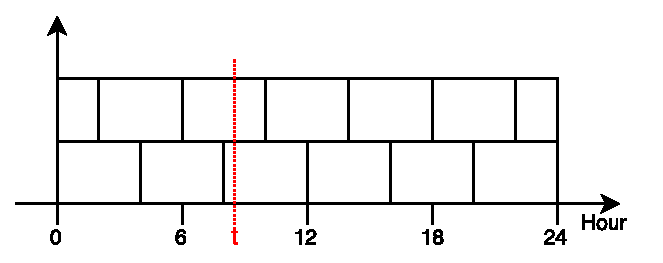
\includegraphics[]{figures/300-time-slots.pdf}
	\caption{Example of shifted time slots used in the entropy analyser module.}
	\label{fig:concept:time-slots}
\end{figure}

\begin{comment}
\begin{itemize}
	\item cf.~Section~\ref{sec:background:network:novelty:entropy}
	\item statistical approach
	\item base model is trained using distribution of the \gls{pmf}
		\subitem determine statistical distribution per dimension in feature vector
	\item determine distribution for local (per agent) and world view
	\item to incorporate different seasons multiple base models are trained 
	\item the seasonal time range (day, week, year) is separated into slots
	\item amount of slots is doubled with half a slot length offset, so 2 slots apply per time point cf. Figure~\ref{fig:concept:time-slots}
	\item mitigates issues with artificial break on slot change
	\item feature vector
		\subitem source addresses
		\subitem destination addresses
		\subitem priority distribution
		\subitem hop count distribution
		\subitem payload length distribution
		\subitem \gls{apci} usage distribution
	\item entropy/information gain is calculated for the current distribution of the feature vector compared to the respectively base model
	\item individual entropies are summed up and stored in the \gls{influxdb} (additional to the individual entropies)
\end{itemize}
\end{comment}

The Entropy Analyser, relies less on the spatial properties of the vector space, but rather on the statistical.
It uses the information theorem by \textcite{Shannon1948} to calculate the information gain or entropy a new incoming window would provide to a base-model.
The base-model is generated during a dedicated training phase and contains a \glsfirst{pmf} for every dimension of the feature vector. Only the time dimension is excluded, since it is continuous.
Seasonal sensitivity is instead archived, as described in Section~\ref{sec:background:network:features:time}, by diving one period into multiple time chunks. Each of these chunks equates to one sub-model, which represents the activity during this time slot. To reduce hard breaks at the end of each chunk, another set chunks is used shifted by half the chunk length. Hence every point of time with in the season period is within two chunks. (see Figure~\ref{fig:concept:time-slots})

Further, two types of base-line models will be trained: One general world-view and many Agent specific models.
The world-view model is used to identify general abnormal behaviour in the network and can be seen as a general-purpose, less sensitive model.
The Agent specific models, on the other hand, are specialised on the traffic and behaviour unique for one Agent. Therefore, they are able to identify local anomalies, which might be completely normal when seen by another Agent.
Opposed to the proximity based \gls{lof} approach, this could not be modelled as additional dimension in the feature vector.
Even though the Agent is an categorical feature, it is assumed to be totally equal distributed, since all Agents report in the same interval.
Consequently, this feature does not add any additional value to the model and certainly is not able to separate behaviour for different Agents.

During normal operation the entropy is calculated for the feature vector of incoming windows compared to the respectively applying chunks of world-view and the specific Agent model.
The resulting entropies are then stored into the database individually as well as sum. From there the monitoring and alerting system can pick these values up and raise an alert, if the summed entropy raises over a certain threshold.

\section{Monitoring and Alerting}
\label{sec:concept:mon}

\begin{comment}
\begin{itemize}
	\item using \gls{grafana}
	\item visualise basic time series like amount of packets per agent
	\item visualise and monitor output from analyser modules
		\subitem should stay below certain threshold
	\item use internal alerting function
	\item benefits
		\subitem use existing, proven solution
		\subitem gain features for free (auth, alerting, graphing, etc)
		\subitem integrate with metrics from other sources
	\item decoupled from analyse modules
	\item good integration with \gls{influxdb}
\end{itemize}
\end{comment}

The by far most important component of the proposed concept is the monitoring and alerting module.
Its task is to visualise metrics derived from the windows stored in the database directly, as well as to visualise the results from the analyser modules.
Most importantly, it also generates user alerts if values raise above a certain secure threshold, so a system administration can assess the situation and possibly initiate counter measures.
Without a proper monitoring and alerting solution the insights gained by the different Analyser modules would be useless, as it would be difficult for a system administrator to troubleshoot incidents and maintain an overview just using log files.
Consequently, visual representations of certain system characteristics allow and observe the network behaviour easily.
The most obvious visualisation is to plot these values as a time series graph, which allows to estimate the change of a measurement over time.
Additionally, graphs visualising the amount of packets per source or destination address, or the amounts of packets per application could be visualised as bar graph.
Based on these graphs and plots alerting rules and threshold can be defined.
However, the exact visualisation setup and alerting rules should be always adapted to the specific use case and network, so it is merely feasible to provide an example here.

Since the problem of monitoring and alerting is a well solved one, it is very feasible to rely on existing standards and third-party solutions for this task and follow the principle of decoupling modules from each other.
This reduces also the scope of this work, and as a result also the code base which need to be maintained for this project.
Furthermore, most organisation already have an existing monitoring solution. By relying on standards it allows them to easily incorporate measurements from the here proposed concept of monitoring \gls{bas} networks into their existing system and possibly combine them with other metrics.

